\chapter{Einleitung}

Im letzten Jahr habe ich mich damit beschäftigt, wie man mithilfe eines Raspberry Pi Umweltdaten messen, aufzeichnen und auswerten kann. Hierzu verwende ich mehrere Sensoren, die die Lufttemperatur (sowohl im Klassenraum, als auch außen), Luftfeuchtigkeit, Luftdruck und die relative Luftqualität. Diese Daten werden als \gls{CSV} gespeichert und können grafisch und rechnerisch ausgewertet werden.
\todo{genauere Beschreibung des Projekts}
\todo{Nennung des Glossars}
\begin{figure}[h]
  \centering
     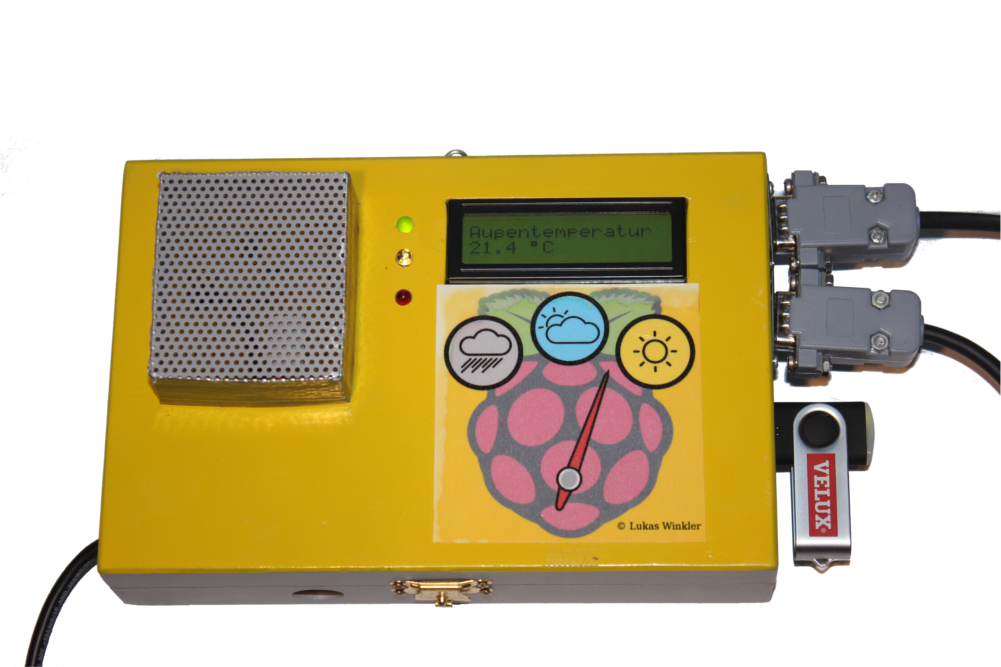
\includegraphics[width=0.9\textwidth]{figures/gesamt.png}
  \caption{Messstation (eigenes Werk)}
  \label{fig:gesamt}
\end{figure}